\ProvidesFile{ch4.tex}[Chapter4]

\chapter{Fluorescence nanoscopy in the study of chromatin organization}
\ix{physics//Physics appendix}

\section{Introduction}

Chromatin is a complex and dynamic structure that packages eukaryotic DNA with histones. Genomic functions such as gene expression, DNA synthesis, and DNA repair are regulated by the higher-order chromatin organization. The chromatin structure and architecture are strictly controlled and constantly remodeled as cells differentiate, divide, and respond to genomic insults \parencite{Auerbach2009,Chien2009,Clapier2009,Misteli2007,Vidi2014}.

While DNA linearly encodes genetic information, serving as a template for RNA and protein production, the temporal and spatial organization of chromatin plays a fundamental role in determining intranuclear activities and gene stability \parencite{Cuvier2017,Dion2013}. For example, local structural fluctuations in nucleosomes on microsecond to second timescales transiently expose buried DNA sites, thus providing temporary access to interaction sites \parencite{Choy2012}. Similarly, chromatin fibers are subject to rapid conformational dynamics \parencite{Li2016}. This intrinsic motion of chromatin directly affects molecular interactions at the local level by dictating the accessibility of DNA for various epigenetic effectors, chromatin regulators, and transcription factors (TFs). Therefore, the nanoscale spatiotemporal profile of chromatin may modulate the interaction of DNA with regulatory molecules, impacting the global patterns of gene expression \parencite{Bintu2018,Boettiger2016,Grant2018,Xu2018}. The kinetics of chromatin are best described by sub-diffusive (or anomalous) diffusion models \parencite{Fierz2019,Shukron2019}.

Most of what we know about local chromatin motion in chromatin remodeling has been derived from ensemble measurements, which provide a population-averaged picture of biochemical access to chromatin. Recent advances using single-molecule approaches have enabled the direct observation of the dynamics of individual molecules, allowing measurement of their respective spatiotemporal localizations and providing functional clues/implications. Particularly, time-course recording of chromatin loci movements provides quantitative measures, allowing us to assess the spatiotemporal dynamics of chromatin and deduce its biophysical properties.

\subsection{Labeling strategies of chromatin}

To successfully illuminate chromatin structure and dynamics, advanced microscopy systems and single-molecule tracking algorithms must be combined with effective labeling techniques. Visualization of chromatin generally involves tagging fluorescent reporters to the central components of the eukaryotic central dogma: DNA, RNA, and proteins. Below, we review various classical and emerging chromatin labeling strategies based on proteins and DNA (summarized in Table 1).

\subsection{Chromatin-associated-protein based labeling strategies}

Core histones (H2A, H2B, H3, and H4), the fundamental units of chromatin tightly wrapped by DNA molecules, are common targets for imaging. In fixed cells, chromatin-associated proteins can be visualized through immunostaining with antibodies \parencite{Conic2018,Ricci2015,Xu2018}. In live cells, histones can be directly fused with fluorescent proteins (FPs) \parencite{Belmont2001,Das2003,Kanda1998}. However, this method faces limitations in controlling labeling density, making it less quantitative for highly expressed proteins.

Photo-active fluorescent proteins (PAFPs) have been developed to address this limitation, allowing real-time quantitative characterization of protein clustering. This method can be combined with other technical strategies such as single-molecule tracking and super-resolution imaging \parencite{Cisse2013,Manley2008,Nozaki2017}. For instance, the Zhuang lab engineered mMaple2 and mMaple3, which showed substantially reduced dimerization tendencies, allowing live-cell imaging for up to 5 hours without detectable phototoxicity or photobleaching \parencite{Wang2014,Baker2010}. Alternatively, histone labeling in live cells can utilize prevalent self-label tags \parencite{Liss2015,Stagge2013}, such as Halo Tag, Snap Tag, CLIP tag, and TMP Tag, which offer advantages like small size, brightness, photostability, monomerization, and adjustable fluorescent dye concentration, demonstrating superior performance in single-molecule imaging \parencite{Grimm2017,Nagashima2019,Nozaki2017}.

Other genomic elements can also be fluorescently labeled to assess structure and dynamics, including telomeres \parencite{Avogaro2018}, centromeres \parencite{Avogaro2018,Gasser2002}, H-NS or HU in E. coli \parencite{Wang2011}, heterochromatin proteins \parencite{Hu2013}, and transcription factors (TFs) \parencite{Elf2007,Gebhardt2013}. Despite their stability and efficacy, protein-based labeling methods have drawbacks, such as being suitable only for global or non-specific investigations and the potential for labeling artifacts due to overexpressed FPs.

\subsection{DNA-based labeling strategies}

\subsubsection{Non-sequence specific}

Several cell-permeable DNA dyes, including Hoechst \parencite{Green2017}, 4′,6-diamidino-2-phenylindole (DAPI), YOYO-1, and DRAQ5, strongly bind to DNA, offering simple labeling methods with excellent photostability in fixed cells. Fluorescently labeled dNTPs, which form the DNA backbone, can also demonstrate chromatin structure \parencite{Bu2019}. However, these fluorescent DNA dyes generally lack specificity, which is crucial for elucidating how DNA structure affects its functional outcomes.

\subsubsection{Sequence specific}

Fluorescence in situ hybridization (FISH) has been developed to detect and locate sequence-specific DNA/RNA in fixed cells using probes complementary to the target sequence \parencite{Bayani2004,Beliveau2015}. Despite its advancements, FISH does not elucidate dynamics in living environments.

Locus-specific labeling in live cells remains in high demand. This has been achieved through either inserting artificial DNA sequences next to target genes, such as the repressor–operator array system (Lac operator (LacO) and Tet operator (TetO) systems), or modified genome-editing tools with inactive nucleases like zinc finger proteins (ZFPs), transcription activator-like effectors (TALEs), and clustered regularly interspaced short palindromic repeats (CRISPRs). The LacO-LacI-FP and TetO-TetI-FP systems are derived from the lactose and tetracycline operons of E. coli, respectively. Lac and Tet repressor proteins fused to FPs serve as tracking foci, recognizing repressor tandem repeat sequences inserted next to the position of interest \parencite{Ding2017,Loiodice2014}. Multiple systems and repressor segments can be used simultaneously in a single cell to enhance system multiplicity and fluorescent amplification \parencite{Backlund2014,Roukos2013,Tasan2018}.

Point accumulation for imaging in nanoscale topography (PAINT) techniques are attractive for single-molecule localization microscopy due to their lack of restriction by photon budget. First demonstrated by Jungmann et al. in 2010 \parencite{Jungmann2016}, DNA-based PAINT has been explored and improved over the past decade. Quantitative PAINT (qPAINT), Forster resonance energy transfer PAINT (FRET-PAINT) \parencite{Jungmann2016}, and Exchange PAINT have been developed to generalize the use of DNA origami to reveal cellular interactions, although off-target challenges remain \parencite{Nieves2018}. Additionally, the ParB-INT system can similarly insert a ~1 kb INT element, providing a strong signal without interfering with chromatin dynamics and transcription \parencite{Saad2014}. Nonetheless, any intrusive DNA insertion can potentially perturb function and alter chromatin locus position and mobility. Non-intrusive methods such as ZFPs, TALEs, and CRISPR-dCas9 avoid these constraints, operating without artificial DNA insertion \parencite{Chen2016,Lindhout2007,Ma2013}. These systems rely on modular proteins with specific DNA recognition, where endonuclease-deficient proteins are usually fused with FPs as detectable signals. Among these strategies, CRISPR imaging systems are gaining attention. Chen et al. re-engineered the type II system to visualize both repetitive elements in telomeres and non-repetitive MUC4 \parencite{Chen2013}. For multicolor imaging within the CRISPR system, one strategy is to use fluorescent Cas9 orthologs from different bacterial species simultaneously, such as Streptococcus pyogenes (SpCas9), Neisseria meningitidis (NmCas9), and Streptococcus thermophilus (St1Cas9) \parencite{Ma2015}. Another alternative strategy involves engineering sgRNA into a scaffold RNA (scRNA) to encode information about the gene of interest and multiple fluorescent reporters \parencite{Zalatan2015}. Recent modifications to CRISPR imaging systems, such as CRISPR-display \parencite{Shechner2015} and CRISPR-rainbow \parencite{Ma2016}, suggest promising applications for investigating chromatin organization and visualizing genome instability and rearrangement \parencite{Chen2016}.


\subsection{Instrumentation for chromatin imaging}

Among many factors that determine the accuracy of chromatin loci movement, spatial resolution is the parameter that dominates the reliability of downstream biophysical analysis \parencite{Burov2013}. Therefore, for most reported work in intranucleus chromatin imaging, objectives with high numerical aperture (N.A. > 1.2) are employed. As indicated in the previous section, multiple fluorophores are used in chromosome labeling strategies to ensure adequate fluorescent signal; consequently, there are few limitations on imaging modalities, and various microscopes can be used for chromatin imaging.

For many intranucleus imaging experiments, an epi-illumination fluorescent microscope equipped with a modern camera (EMCCD or sCMOS) (Figure 1A) can provide time-course recording of live cells. Additionally, emerging LED light sources are replacing laser excitation in these microscopes, which significantly reduces the cost of the microscope \parencite{Albeanu2008,Hattori2009,Zheng2013}. Another widely applicable imaging system for chromatin imaging is the confocal microscope (Figure 1B), which offers good z-sectioning capability to reduce out-of-focus background. However, the applicability of confocal microscopy for chromatin motion is due to the relatively slow motion in the nucleus (D < 0.001 μm²/s) \parencite{Shukron2019}. Despite its advantages, confocal microscopy suffers from intrinsic limitations such as photo-bleaching/photo-toxicity and poor temporal resolution, which restrict their applications for sensitive chromatin imaging at the single-molecule level.

The usual alternative to epi-illumination microscopes is total internal reflection fluorescence microscopy (TIRF) (Figure 1C), which can capture photons from a single fluorescent molecule. However, it is not suitable for chromatin imaging in the nucleus due to its poor penetration depth (~200 nm).

Emerging light sheet illumination offers solutions to the aforementioned challenges and achieves a balance among spatiotemporal resolution, photo-bleaching effects, and background reduction (Figure 1E). In 2008, a simple yet efficient light sheet illumination method was proposed to generate a highly inclined and laminated optical sheet (HILO) for single-molecule imaging \parencite{Tokunaga2008}. The high spatial resolution can be retained thanks to the high N.A. objective, and HILO illumination significantly reduces total illumination doses on the cell, though it results in a largely reduced field of view (Figure 1D). Since then, light sheet illumination has garnered tremendous attention for its advantages in reducing phototoxicity, enhancing sectioning capability, and enabling live-cell three-dimensional (3D) imaging. Early development of light sheet microscopy, using two orthogonal objectives (N.A. ~ 0.65) for excitation and/or emission, has shown great performance for 3D imaging of tissues, embryos, and organs \parencite{Keller2015,Keller2010,Keller2008,Tomer2011}. However, its application in single-cell and even single-molecule imaging was limited by geometric hindrance when using two high N.A. objectives. Recent efforts have focused on developing new light sheet modalities for single-cell 3D imaging. An AFM cantilever was initially used to reflect the illumination light sheet by 90 degrees to bypass geometric hindrance \parencite{Gebhardt2013}. A similar idea was proposed using a microfabricated reflecting chip next to the sample reservoir \parencite{Galland2015}. Both approaches can generate a thin sheet of light with a beam waist of ~1 μm. Furthermore, the lattice light sheet (LLS) microscope, which generates the light sheet with a Bessel beam, significantly reduces the thickness of the light sheet to 300 nm \parencite{Chen2014}. The LLS has demonstrated superior performance in terms of spatial resolution, temporal resolution, phototoxicity, and sensitivity \parencite{Gao2019}. However, generating optical lattices requires a complex, expensive, and lossy optical train. A recent study proposed a simple and universal optical process, described by a mathematical theorem as field synthesis, to create any type of light sheet, including the lattice light sheet \parencite{Chang2019}. This approach can be integrated with any light sheet imaging system to enable lattice light sheet imaging.

The further development of imaging modalities for chromatin imaging will aim at a light sheet imaging technique that balances various imaging parameters and provides time-course recording of chromatin motion in 3D. Generally, chromatin can be modeled as beads on a string. To determine polymer models that accurately reflect the behavior of chromatin inside the nucleus, one must compare extracted physical parameters from real experimental chromatin data with those predicted from the model. However, physical models often fail to infer actual chromatin dynamics due to inconsistencies between modeling and experiments. This discrepancy arises because 2D imaging data cannot offer positional information of chromatin motion in 3D, whereas physical modeling is in 3D. A recent study by the Misteli group compared 2D and 3D distance measurements in the cell nucleus \parencite{Finn2017}. While 2D measurements (i.e., positions or trajectories projected in a single plane) are practical and generally well-suited for flat nuclei in monolayer cell cultures, 3D measurements are necessary to improve accuracy, particularly for round nuclei (e.g., in 3D cultures) where the relationship between 2D and 3D distances deteriorates, and for short distances (<5 μm) where the average 2D/3D discrepancy is ~30 percent \parencite{Finn2017}. Moreover, nuclear inhomogeneity in all 3 dimensions must be considered. For motion measurements, the 2D/3D discrepancy of ~30 percent might not be very significant, but considering local fluctuations of ~50 nm, the 3D nature cannot be ignored.

It is worth noting that the imaging instrumentation and analysis methods discussed here share many similarities with localization-based super-resolution microscopes, such as Fluorescence Photoactivation Localization Microscopy (PALM or fPALM) and Stochastic Optical Reconstruction Microscopy (STORM). Advances in super-resolution imaging will also benefit intranuclear chromatin imaging. For example, aspheric optics were initially utilized in super-resolution imaging to convert the z-axis position of a single molecule into a distorted point spread function (PSF) on the x-y plane using a cylindrical lens \parencite{Huang2008}. This method was further developed in single-molecule imaging/tracking to register the 3D position of a moving molecule through a rotational PSF \parencite{Greengard2006,Pavani2009,Badieirostami2010,Thompson2010}. Additionally, applying super-resolution imaging to live-cell single-molecule imaging produces high-density trajectories of molecules, enabling the integration of biophysical analysis such as stochastic models of nonequilibrium motions to recover forces, subcellular organizations, diffusion kinetics, and other biophysical features at unprecedented spatiotemporal resolution \parencite{Hoze2012,Holcman2015,Hoze2015}.

Recent progress in quantitative super-resolution imaging, such as qPAINT \parencite{Jungmann2016,Culley2018,Mockl2019}, is expected to be the next booster for live-cell chromatin imaging.

\subsection{Trajectory linking}

 A diverse set of particle tracking algorithms utilize probabilistic models of particle motion in order to add detected particles to existing tracks. Perhaps the most fundamental particle tracking method in this category is the nearest neighbor (NN) linking algorithm first introduced by Crocker and Grier. The algorithm constructs particle trajectories by assuming that the ensemble consists of non-interacting indistinguishable particles undergoing Brownian motion. As a result, the displacement of each particle follows a Gaussian distribution, parameterized by the diffusion coefficient and the time-resolution of the sequence. The most probable assignment of detected particles to existing tracks can then be found by maximizing the product of several Gaussian distributions \parencite{Crocker1996}. An attractive feature of this algorithm is that it is relatively simple to implement; however, assumptions that underlie the method impose limitations. In particular, if a typical displacement $\delta$ in one time step is comparable to the typical inter-particle spacing, tracking becomes highly error-prone \parencite{Crocker1996}. In other words, when particles are simultaneously densely distributed and undergoing fast diffusion, the algorithm can fail to build accurate trajectories due to the ambiguity introduced by overlapping trajectories. This also applies to the limit of low frame rates when small displacements are not recorded by the sensor. Importantly, the method alone cannot handle cases where particles disappear permanently, temporarily disappear due to blinking, photo-bleaching, or missed localization \parencite{Sbalzarini2005}.

\subsection{Quantitative analysis of particle motion}

Based on trajectory data, quantitative information regarding the motion of the particle can be extracted (Figure 2D). It is important to note that the chromatin structure is highly complex and cannot be exactly represented by the diffusion of individual particles. However, by treating each fluorescent foci as a point mapped in space and time, we can determine whether the motion is constrained (sub-diffusion), super diffusion, or follows normal diffusion. Thus, by using only position data (via particle tracking algorithms) and frame rate, we can uncover the following parameters.

The most common method to analyze single particle trajectories is to calculate the mean square displacement (MSD), which represents the scaling of the average squared displacement from the origin as a function of time:

\begin{equation}
\text{MSD} = \frac{1}{N} \sum_{i=1}^{N} \left[ \mathbf{r}(t + \tau) - \mathbf{r}(t) \right]^2
\end{equation}

The sampling time given by $\tau$ is interpreted as the frame rate of the camera. Certain studies have shown that the observed motion varies with different values of $\tau$ \parencite{Amitai2017,Shukron2017a}. Once the MSD curve is established, the effective diffusion coefficient $D$ and the anomalous exponent $\alpha$ values can be obtained by curve-fitting techniques using:

\begin{equation}
\text{MSD}(\tau) = 2mD\tau^\alpha
\end{equation}

where $m$ is the number of dimensions. These parameters reflect the velocity of diffusion and the degree of confinement of individual particles, respectively. Importantly, different parameter values allow for further interpretation and classification of different diffusion modes of particles \parencite{Wasim2018,Zhong2020}.

By comparing the $D$ values of all particles within the nucleus, spatial heterogeneity can be clarified. Meanwhile, different $\alpha$ values can be fitted to different diffusion models. For trajectories with $\alpha = 1$, the motion is considered to be Brownian motion; when $\alpha > 1$, it is said to be directed motion; and $\alpha < 1$ is classified as confined (or immobilized) diffusion.

While the calculation of $D$ and $\alpha$ is particularly reliant on the length of the trajectory and the number of data points, recent investigations have built diffusion color maps of fluorescently labeled histones by computing vast amounts of super-resolution trajectories. This approach aims to reveal mechanisms or interactions in cell biology \parencite{Amitai2017,Barth2020,Nozaki2017}.

\subsection{Polymer models for chromatin dynamics}

\begin{figure}[t]
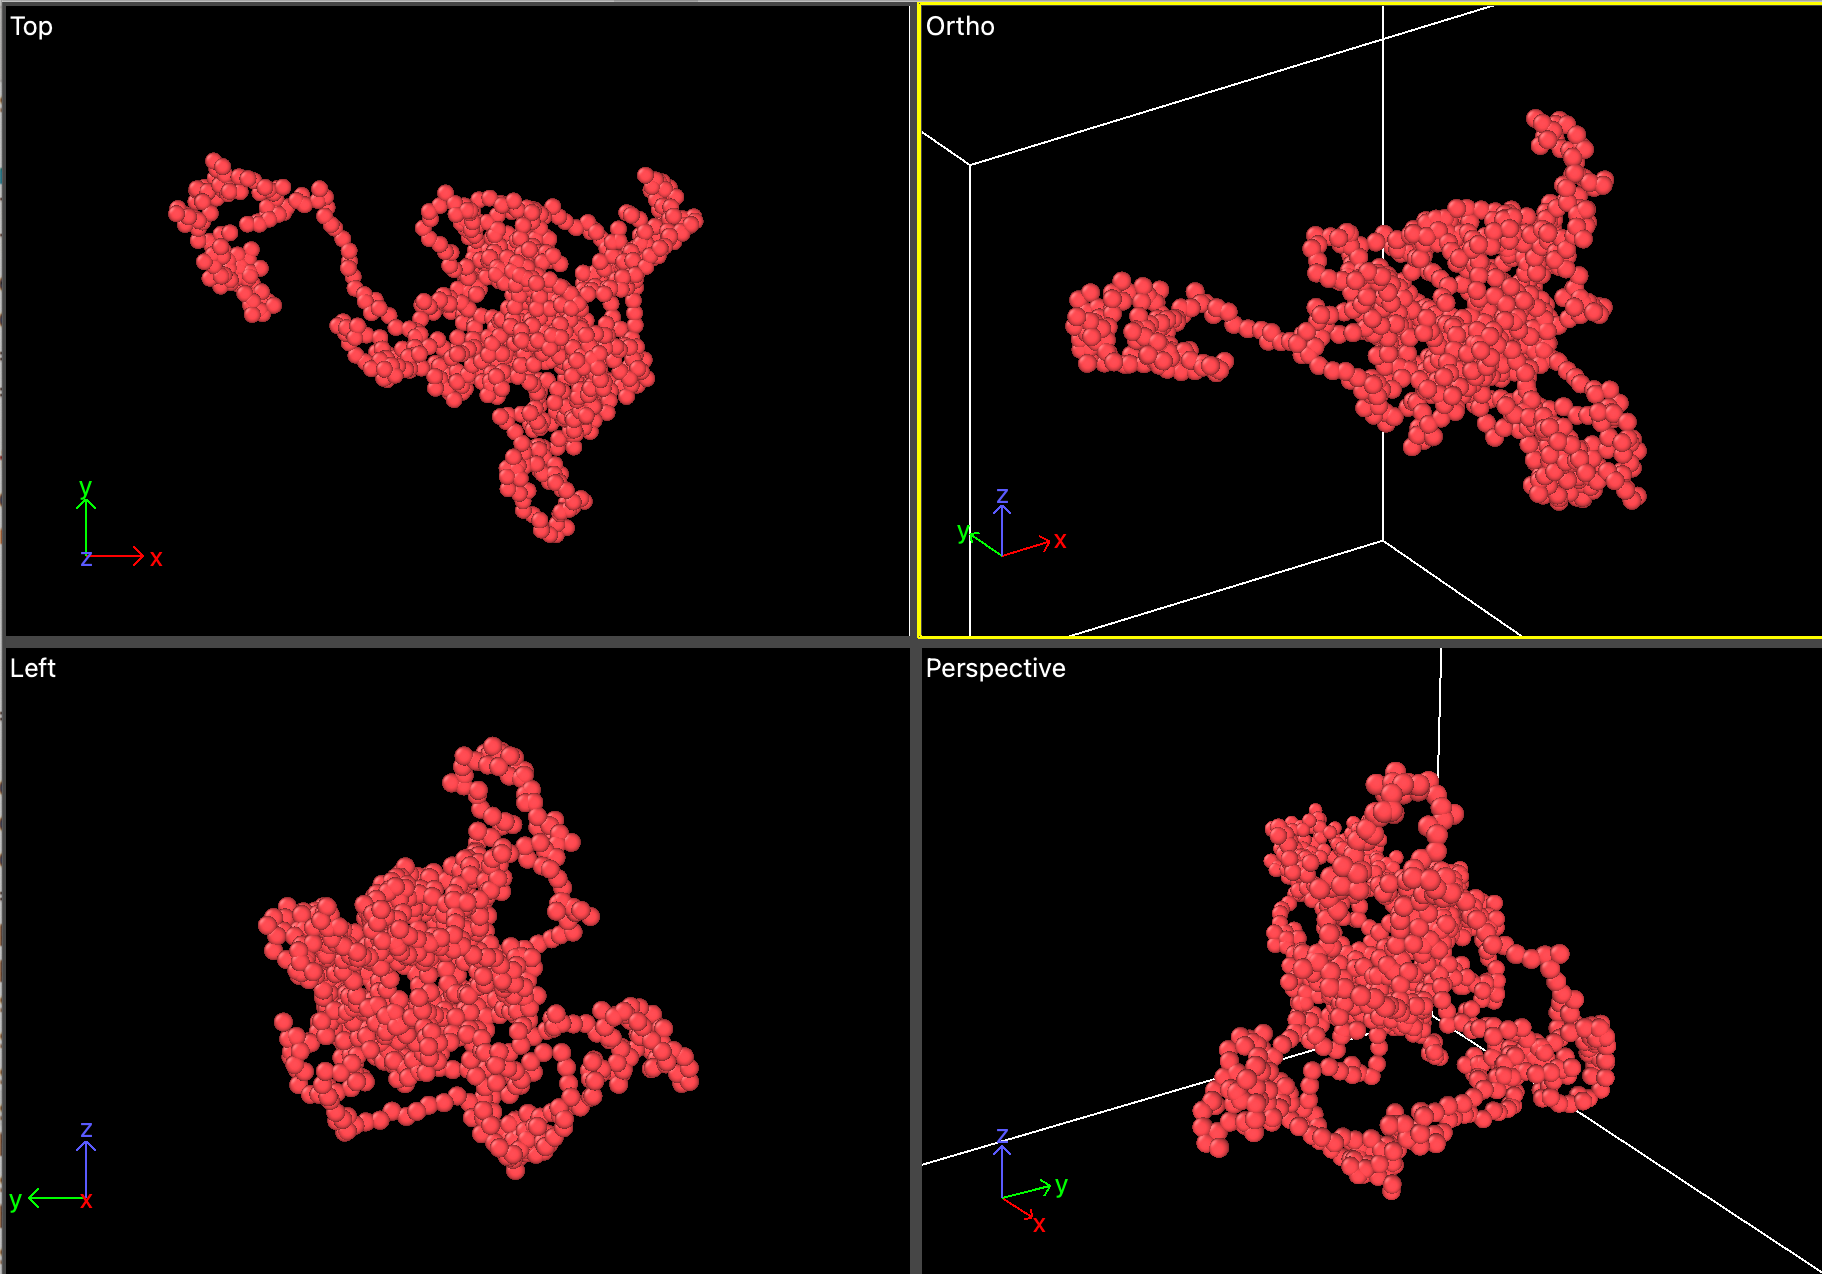
\includegraphics[width=\textwidth]{/Users/cwseitz/git/cwseitz.github.io/docs/phd/brd4/brd4/media/Rouse.png}
\caption{\textbf{Snapshots of the Rouse polymer}. Four perspectives of the Rouse polymer generated with $N=2000$ beads connected with harmonic bonds with equilibrium length $200\mathrm{nm}$. Polymer is initialized with all harmonic bonds at equilibrium}
\end{figure}

\begin{table}[h!]
\centering
\begin{tabular}{|c|c|}
\hline
\textbf{Parameter} & \textbf{Value} \\ \hline
Temperature ($T$) & 310 K \\ \hline
Bond Length ($\sigma$) & $200 \times 10^{-9}$ m \\ \hline
Cutoff Distance & $500 \times 10^{-9}$ m \\ \hline
Spring Constant ($\kappa$) & 90.0 $k_{B}T/\sigma^2$ \\ \hline
Neighbor Distance & $500 \times 10^{-9}$ m \\ \hline
Damping Coefficient ($\gamma$) & $10^{-4}$ \\ \hline
Time Step & 1s\\ \hline
Number of Time Steps & $10^4$ \\ \hline
Number of Atoms & 2000 \\ \hline
\end{tabular}
\caption{\textbf{Rouse polymer parameters}}
\end{table}

It is well-known that the DNA double helix structure consists of millions of base pairs chained together by the sugar-phosphate backbone. DNA, being a molecule built from many similar monomers bonded together, is naturally analyzed using a polymer model. The simplest polymer model for chromatin is the Rouse polymer model, which discretizes it into monomers connected by springs, resembling the string-of-beads structure observed under the electron microscope. Various forces acting on chromatin result in constrained dynamics, leading to significant variability in the anomalous exponent $\alpha$ for the dynamics of a chromatin locus.

To refine the modeling of chromatin properties according to the exponent $\alpha$, the $\beta$-polymer model was introduced. This model accounts for mid-range and long-range interactions between monomers, not just those between the nearest neighbors as in the Rouse polymer model. In this model, $\alpha$ shows a decay curve with distance along the chain. While $\alpha = 0.5$ in the traditional Rouse polymer model, the $\beta$-polymer model can be selected to address cases where $\alpha$ is in the range of 0 to 0.5 \parencite{Amitai2013,Amitai2017,Hajjoul2013}. Thus, local interactions between monomers can be inferred from the anomalous diffusion exponent using this construction.

\begin{figure}[t]
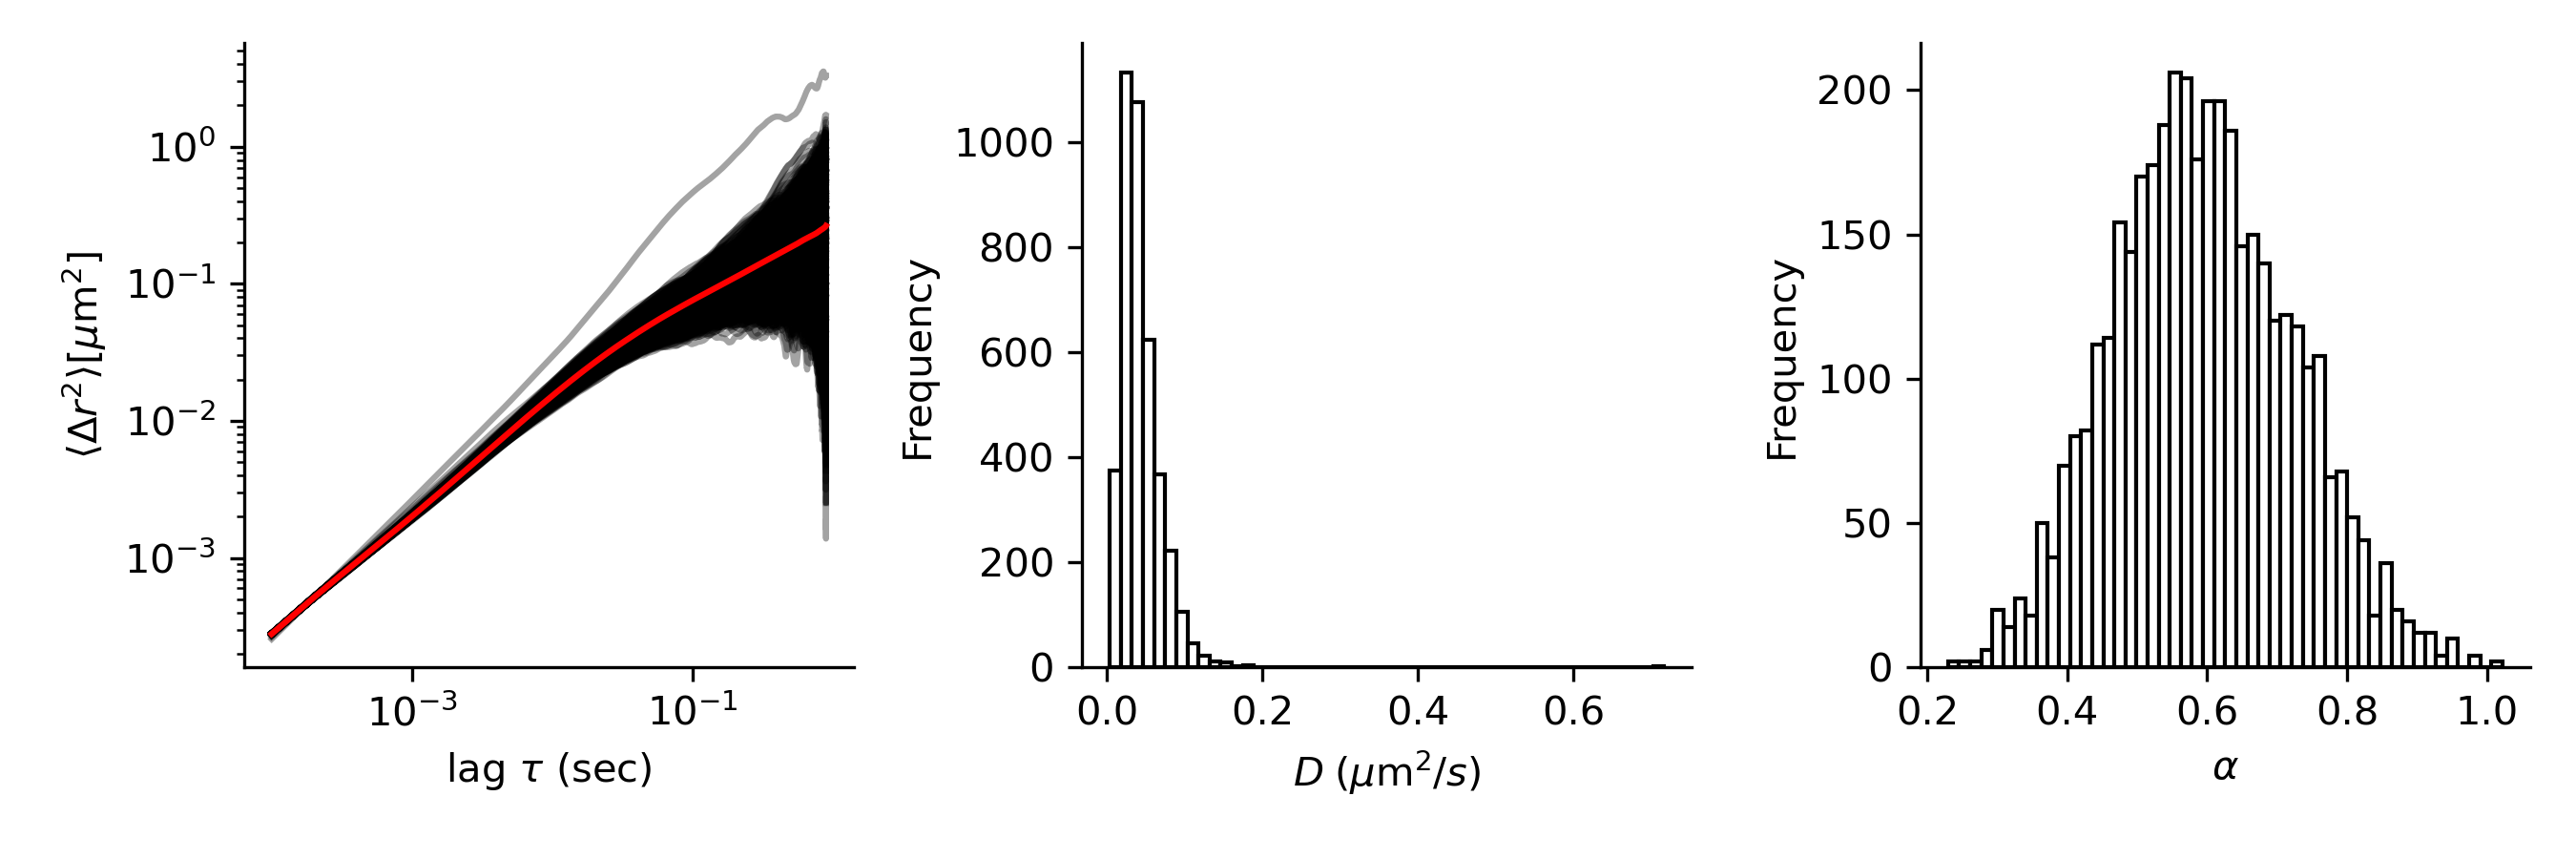
\includegraphics[width=\textwidth]{/Users/cwseitz/git/cwseitz.github.io/docs/phd/brd4/brd4/media/Rouse-Dynamics.png}
\caption{\textbf{Subdiffusive dynamics of the Rouse polymer}. (left) Mean squared displacement (MSD) of individual beads shown in gray, average MSD shown in red. (middle) Histogram of the diffusion coefficient of individual beads. (right) Histogram of the anamalous exponent. Fitting of individual bead MSDs performed by linear regression in log-space using the first 5000 time points}
\end{figure}

Furthermore, as the polymer model usually folds at different spatial scales and generates various sizes of loops, a simulation model adding connectors between randomly chosen non-nearest neighbor monomer pairs, known as the randomly cross-linked (RCL) polymer model, was presented. In this model, $\alpha$ is reduced to below 0.5 by adding connectors. Recent evidence suggests that the number and distribution of connectors impact physical parameters in various ways, but this domain remains underexplored. Notably, the RCL polymer model may be crucial for studying dynamics in processes such as CTCF and cohesion regulating chromatin loop stability \parencite{Hansen2017}. Additionally, sub-diffusion with an exponent $\alpha > 0.5$ can occur in some polymer models, potentially involving different types of forces such as deterministic forces, directed motion, or other monomer interactions (self-avoiding and bending interactions).

\subsection{Super resolution of chromatin nanodomains}

The interplay between chromatin structure and phase-separating proteins is an emerging topic in cell biology with implications for understanding disease states. Here, we investigate the functional relationship between bromodomain protein 4 (BRD4) and chromatin architecture. By combining molecular dynamics simulations with live-cell imaging, we demonstrate that BRD4, when phosphorylated at specific N-terminus sites, significantly impacts nucleosome nanodomain (NN) organization and dynamics. Our findings reveal that enhanced chromatin binding activity of BRD4 condenses NNs, while both loss or gain of BRD4 chromatin binding reduced diffusion of single nucleosomes, suggesting a role for BRD4 in the regulation of nanoscale chromatin architecture and the chromatin microenvironment. These observations shed light on the nuanced regulation of chromatin structure by BRD4, offering insights into its role in maintaining the nuclear architecture and transcriptional activity.

\section{BRD4 regulates the structure of chromatin nanodomains}

The cell nucleus is a densely packed environment with chromatin comprising a dominant component. The compartmentalization of chromatin with other intranuclear components by phase separation is therefore an efficient strategy to ensure precise spatial and temporal coordination of complex dynamics. A growing number of phase separated nuclear bodies have been identified, including transcriptional condensates \parencite{Sabari2018,Hnisz2017}, nuclear speckles \parencite{Brown2008}, and DNA damage repair foci \parencite{Wang2023}; however, the interplay of phase separated condensates with the underlying chromatin structure remains poorly understood. Transcriptional condensates have been identified as an ideal model to study the kinetic and thermodynamic contributions of chromatin substrate binding, as the ability of transcriptional activators to both condense and bind chromatin is well established \parencite{Sabari2018,Wagh2021,Plys2018,Strom2024,Ma2021}. Here, we extend this effort by investigating the regulation of chromatin structure by phase separated transcriptional condensates. We focus on the BRD4 protein - a well-studied transcriptional activator that localizes to acetylated chromatin sites \parencite{Wu2018}, recruits pTEF-b, and initiates transcription of key genes involved in signal response, immunity, and oncogenesis \parencite{Itzen2014}.

The BRD4 long isoform is characterized by structured N-terminal tandem acetyl-lysine binding bromodomains and an extra-terminal domain, connected by intrinsically disordered regions \parencite{Han2020}. Perhaps the most fundamental of BRD4 functions is the ability to bind to acetylated chromatin through bromodomain 1 (BD1) and bromodomain 2 (BD2) that are in tandem within the N-terminal part of the protein. BRD4 inhibitors such as (+)-JQ1 competitively bind to the acetyl-binding pocket of BRD4, displacing BRD4 from chromatin \parencite{Filippakopoulos2010}. It is also well known that BRD4 association with acetylated chromatin is enhanced by casein kinase II (CK2)-mediated phosphorylation of seven N-terminus phosphorylation sites (NPS), followed by intramolecular rearrangement of BRD4 protein and/or BRD4 dimerization \parencite{Wu2013,Malvezzi2021}.

\begin{figure}[t]
\centering
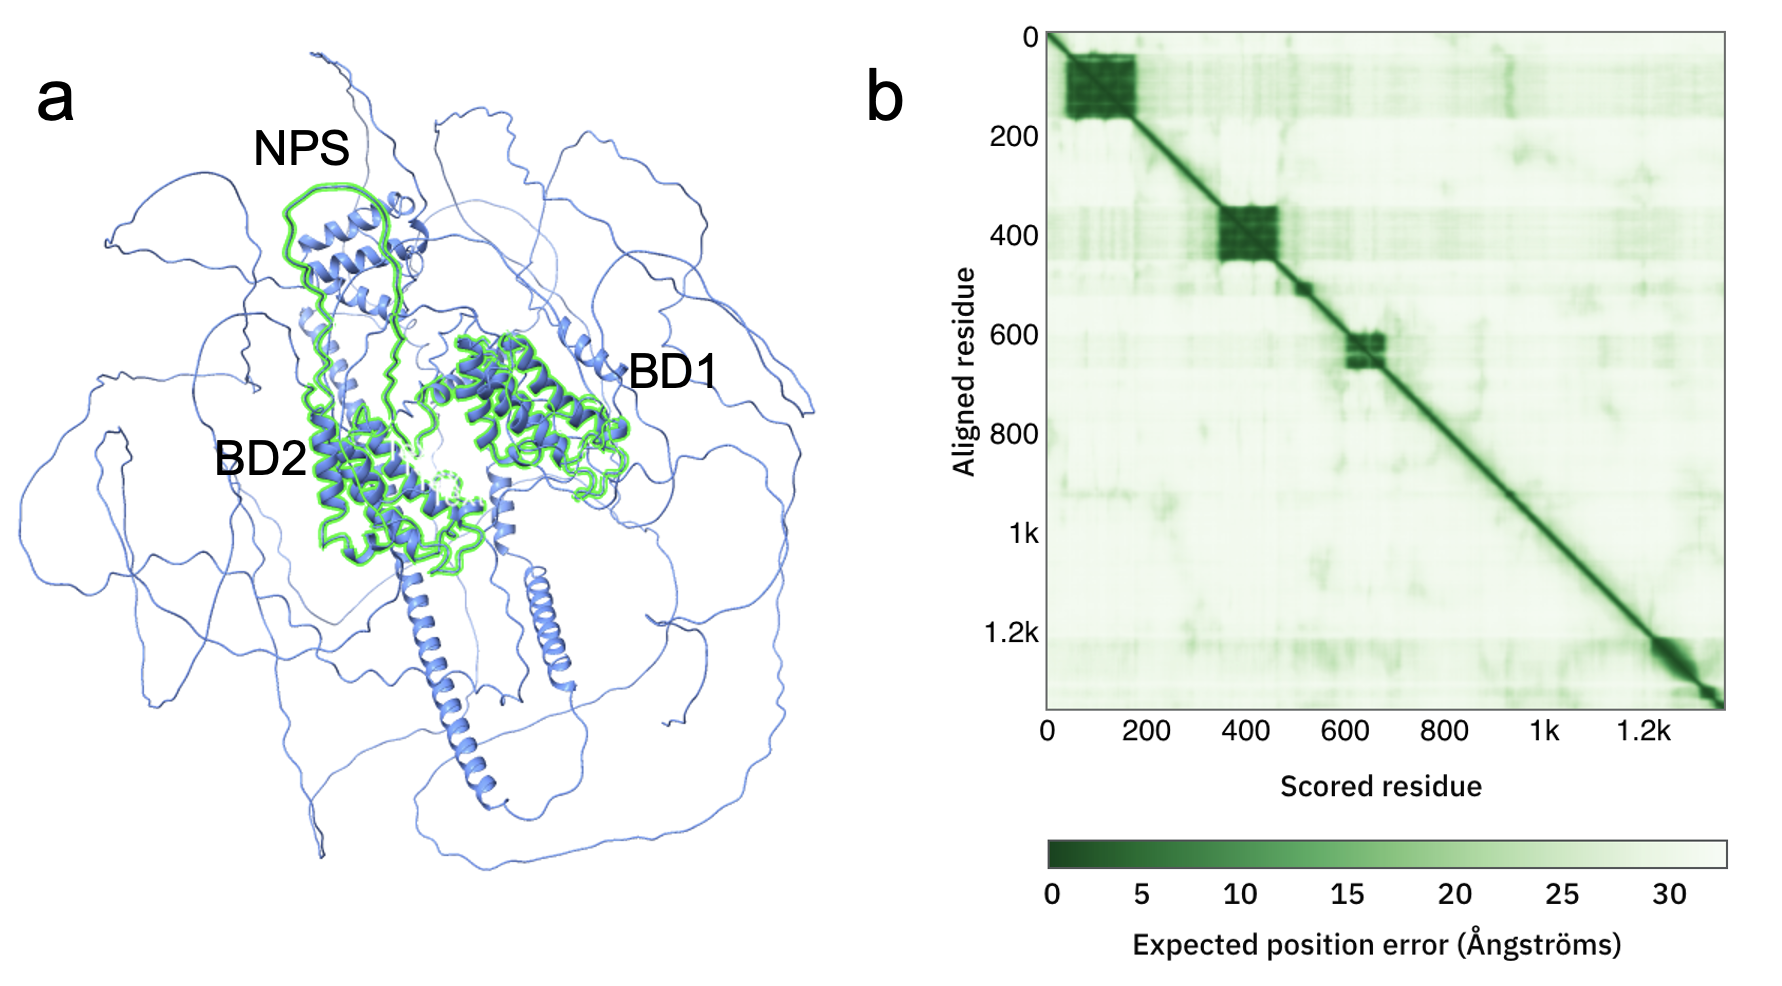
\includegraphics[width=14cm]{/Users/cwseitz/git/cwseitz.github.io/docs/phd/brd4/brd4/media/Structure.png}
\caption{\textbf{Bromodomain protein 4 (BRD4) structure prediction}. (a) AlphaFold predicted structure of BRD4 long isoform (blue) with bromodomain 1 (BD1) aa58-163, bromodomain 2 (BD2) aa349-456, and N-terminus phosphorylation sites (NPS) aa462-506 highlighted in green. (b) Heat map of expected position error in AlphaFold prediction}
\end{figure}

Recent studies have demonstrated that BRD4 is present in discrete nuclear bodies that occur at super-enhancers, which exhibit properties of other well-studied biomolecular condensates, including rapid recovery of fluorescence after photobleaching and sensitivity to 1,6-hexanediol, which disrupts liquid-like condensates \parencite{Sabari2018}. Both BRD4 long and short isoform are found in phase separated condensates in the nucleus and are associated with active gene transcription1. Importantly, CK2-mediated NPS phosphorylation state regulates chromatin binding activity of BRD413 as well as BRD4 phase separation \parencite{Han2020}. This has led to the conclusion that phosphorylation of BRD4 inhibits interaction with chromatin and reduces phase separation, while remaining necessary for active gene transcription. Moreover, phosphorylated and unphosphorylated BRD4 form different molecular associations – transient polyvalent associations of unphosphorylated BRD4 contrast with the stable dimeric interaction and chromatin binding of phosphorylated BRD4 \parencite{Malvezzi2021}. We therefore speculated that BRD4 chromatin binding may be necessary for maintaining NN structure and single nucleosome dynamics. 


\section{Results}

\subsection{Colocalization of BRD4 mutants with nucleosome nanodomains}

To address the role of BRD4 binding and phase separation on chromatin structure, we express FLAG-tagged BRD4 mutants with NPS or bromodomain mutations in HeLa cells and measure their effects on chromatin organization. In particular, we express a constitutively phosphorylated (7D mutant), constitutively unphosphorylated (7A mutant), and bromodomain-deactivated (BD mutant) protein (Figure 1a,b). Colocalization analysis of FLAG-tagged 7A/7D BRD4 mutants with NNs using nearest neighbor distance distribution function G(r) showed an obvious colocalization of these mutants with NNs with respect to complete spatial randomness. 

\begin{figure}[t]
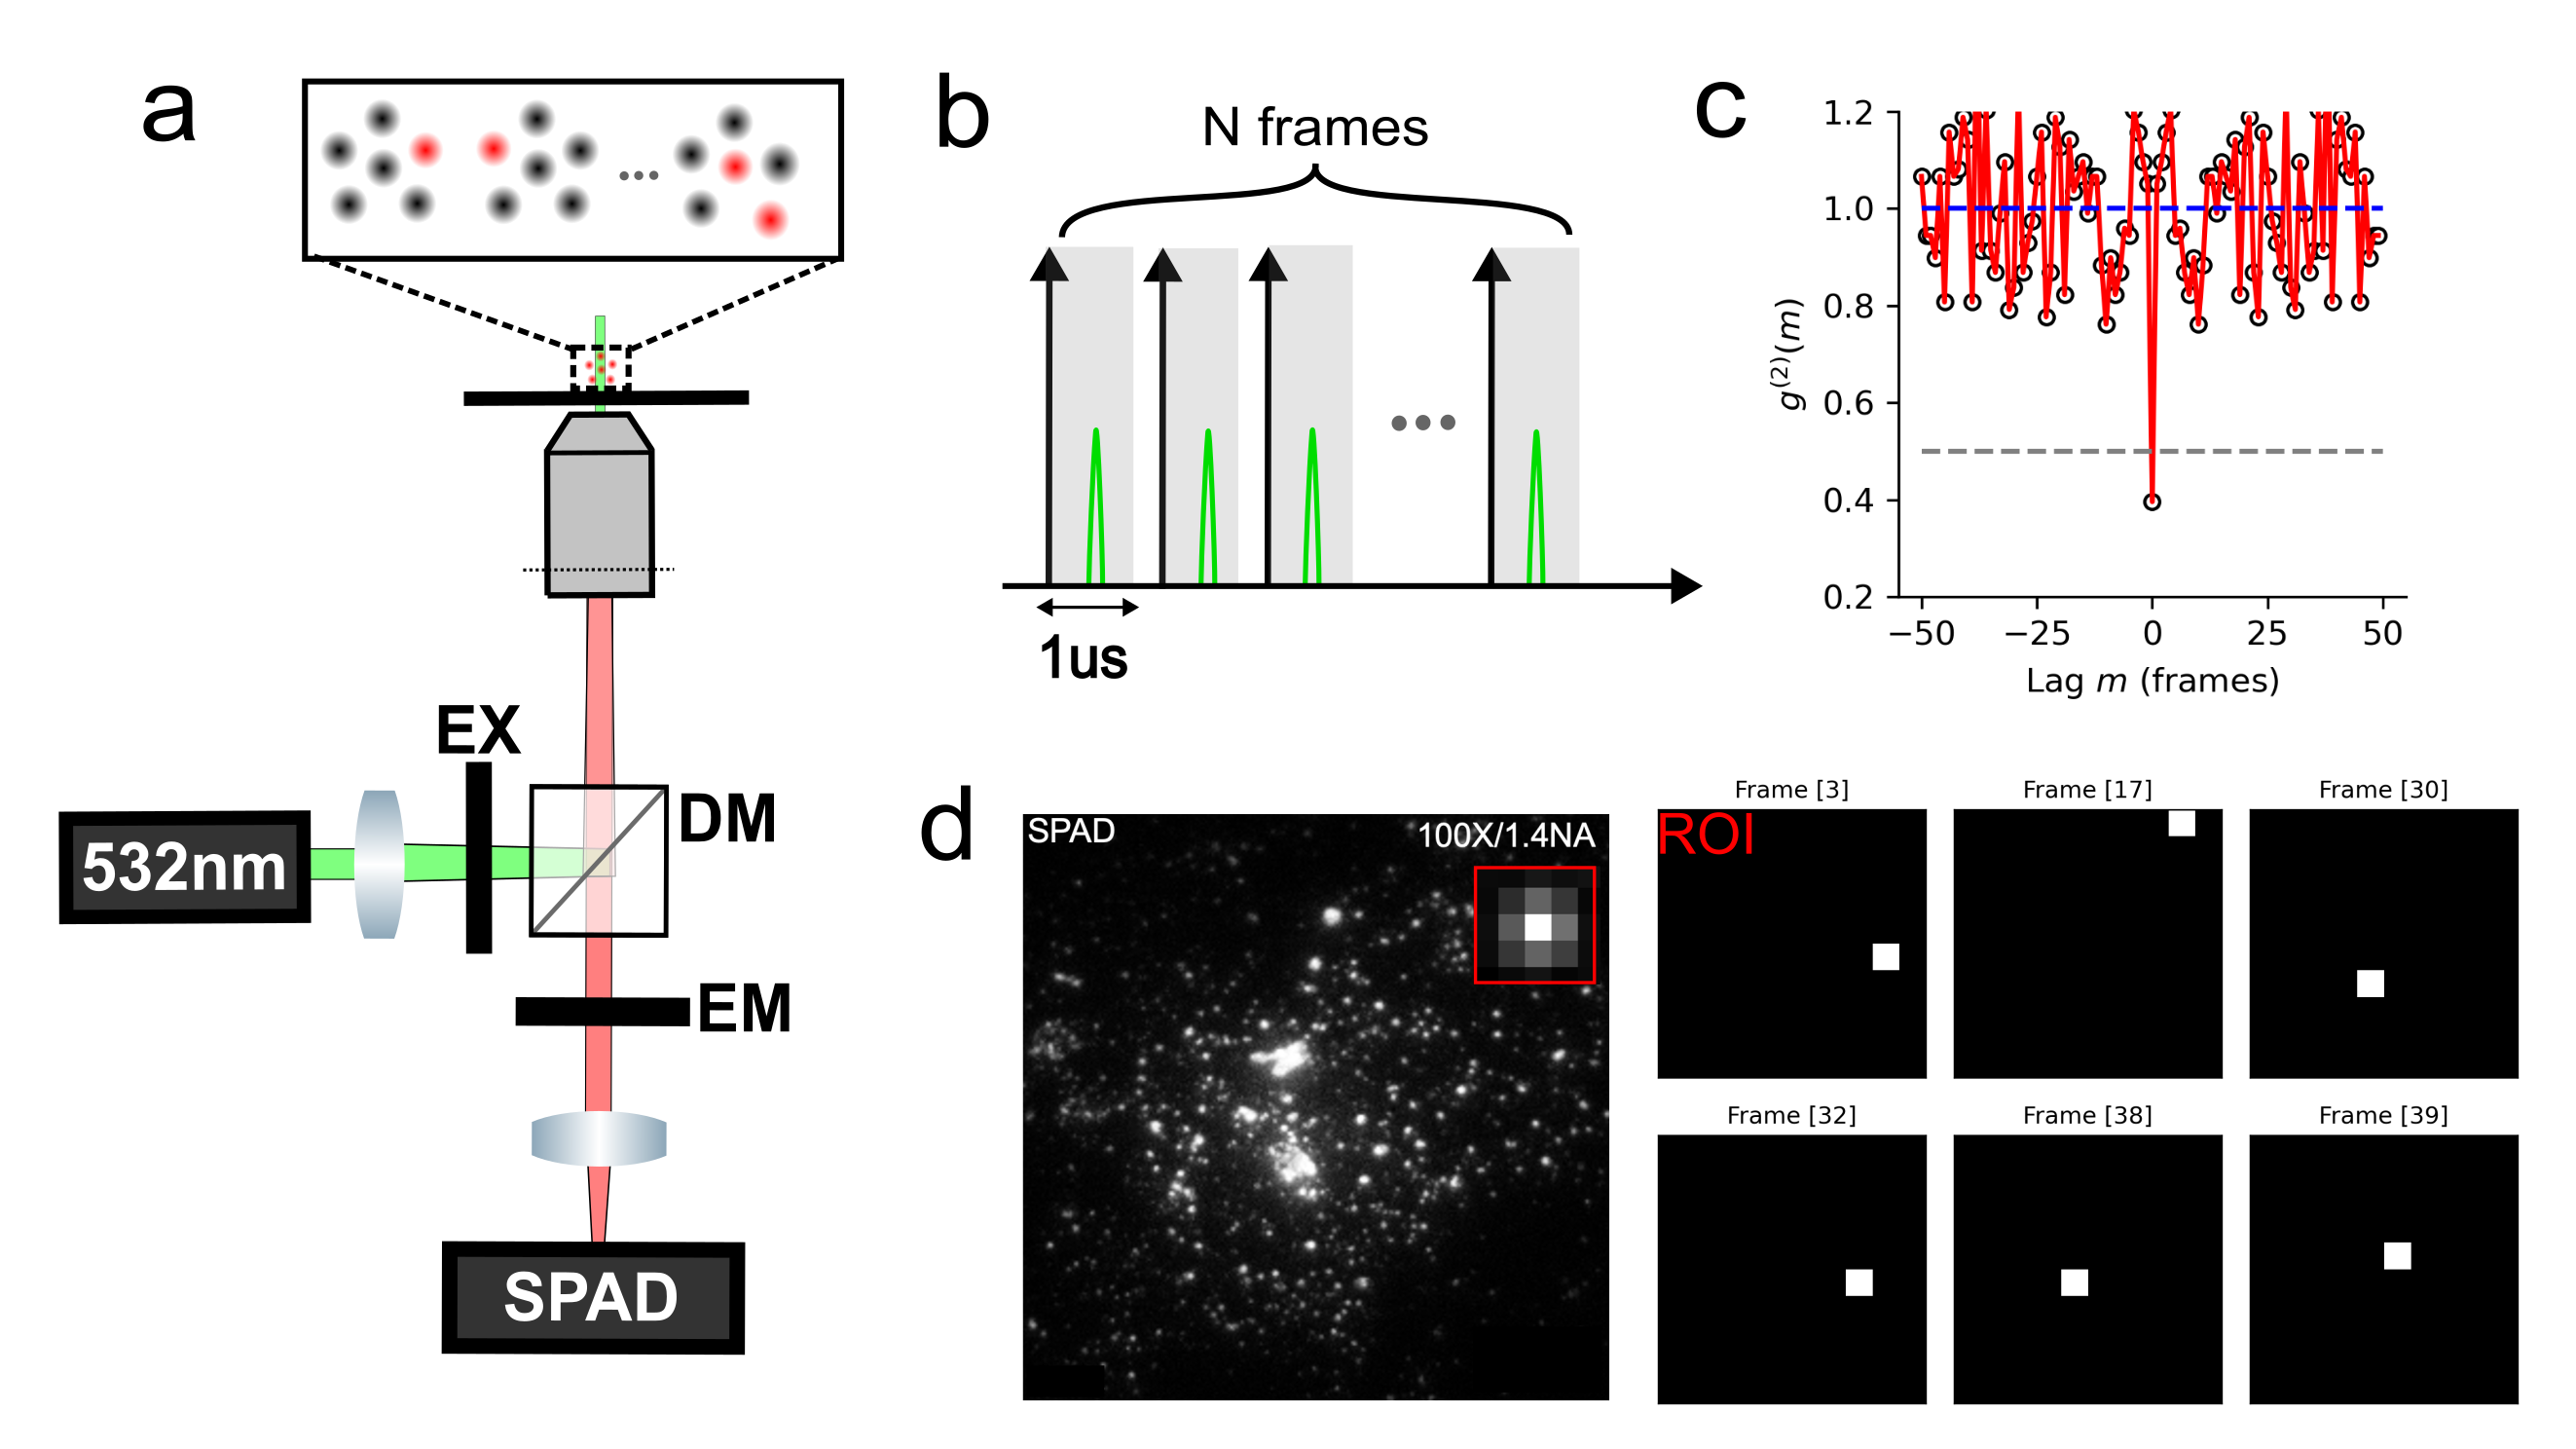
\includegraphics[width=\textwidth]{/Users/cwseitz/git/cwseitz.github.io/docs/phd/brd4/brd4/media/Figure-0.png}
\caption{\textbf{Exogeneous BRD4 mutants colocalize with nucleosome nanodomains}. (a) Schematic of the BRD4 protein sequence and mutations in the NPS region shown in red. (b) Anti-FLAG western blot of bulk expression of BRD4 mutants. (c) Immunofluorescence of BRD4 mutants and combined immunofluorescence of FLAG-tagged BRD4 mutants with JF646-tagged H2B (d) Cumulative nearest neighbor distribution function, averaged over N=20 cells for 7A (blue) 7D (red) mutants, relative to the function under complete spatial randomness (dashed). }
\end{figure}
	
\subsection{Chromatin structure and dynamics}

To assess the functional role of BRD4 in maintaining the NN environment, we interrogated the dynamics of NNs, as well as their structure, in the presence of BRD4 mutants. Histone H2B was tagged with HaloTag \parencite{Los2008} (H2B-Halo), to which a fluorescent ligand JaneliaFluor646 (JF646) can bind specifically in a living cell. Low concentrations of JF646 were used to obtain sparse labeling of nucleosomes for single-nucleosome imaging (Figure 2a,b). JF646-labeled nucleosomes in Hela cells were recorded at 10fps (∼200 frames, 20 s total) and a reduced diffusion coefficient was measured in cells expressing 7A, 7D, and BD mutants, with respect to cells expressing the wild-type BRD4 protein (Figure 2c,d). We then conducted super resolution imaging of nucleosome nanodomains using direct stochastic optical reconstruction microscopy (dSTORM) by promoting JF646 fluorescence intermittency with a cysteamine buffer (Figure 3a,c). JF646 is known to exhibit a transient fluorescent state lasting tens to hundreds of milliseconds and stable dark state lasting hundreds of milliseconds to seconds \parencite{Grimm2015}. Two color imaging of H2B-Halo-JF646 and GFP-tagged BRD4 shows that BRD4 and NNs form complementary biomolecular condensates in the nucleus, consistent with current models of BRD4 chromatin reading mechanism (Figure 3b). Ensemble averages of Besag’s L-function showed an increase in NN compaction in cells expressing the 7D BRD4 mutants, while all other groups were consistently indistinguishable from WT cells (Figure 3d).  

\begin{figure}[t]
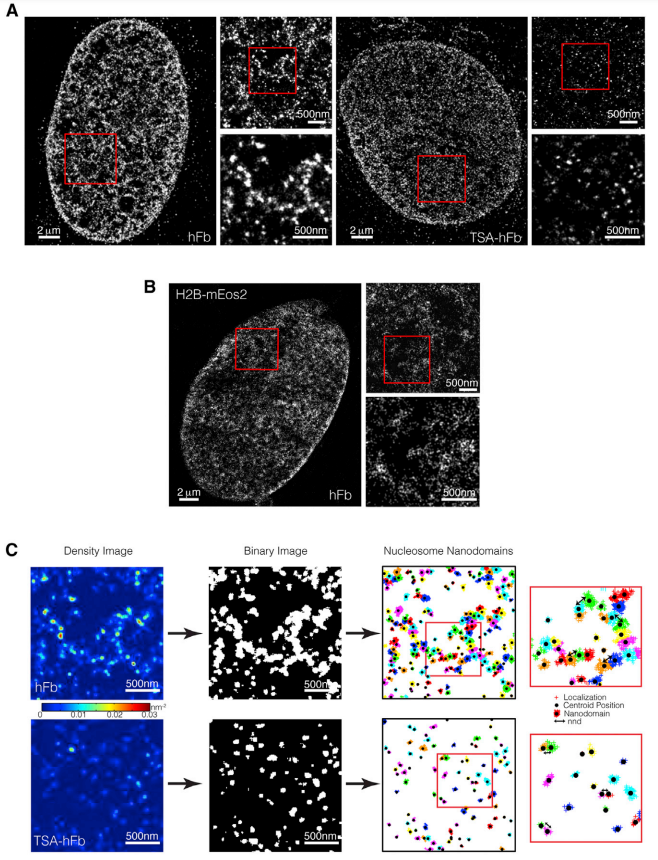
\includegraphics[width=\textwidth]{/Users/cwseitz/git/cwseitz.github.io/docs/phd/brd4/brd4/media/Figure-1.png}
\caption{\textbf{Strong multivalent chromatin binders reduce diffusion of nucleosome nanodomains}. (a) Heteropolymer model of chromatin consisting of A-type, B-type, and C-type particles. (b) Interaction potentials $U_{BC}(r_{ij})$ of multivalent chromatin binders with B-type chromatin beads. (c,d) Example free heteropolymer and heteropolymer with a number density of C-type particles of $\rho=500/\mu m^3$ in a 10um periodic box. (e) Scaled diffusion coefficient $D$ for various chromatin binding energies of C-type particles, averaged over ten independent simulations, with burn-in discarded.}
\end{figure}

\begin{figure}[t]
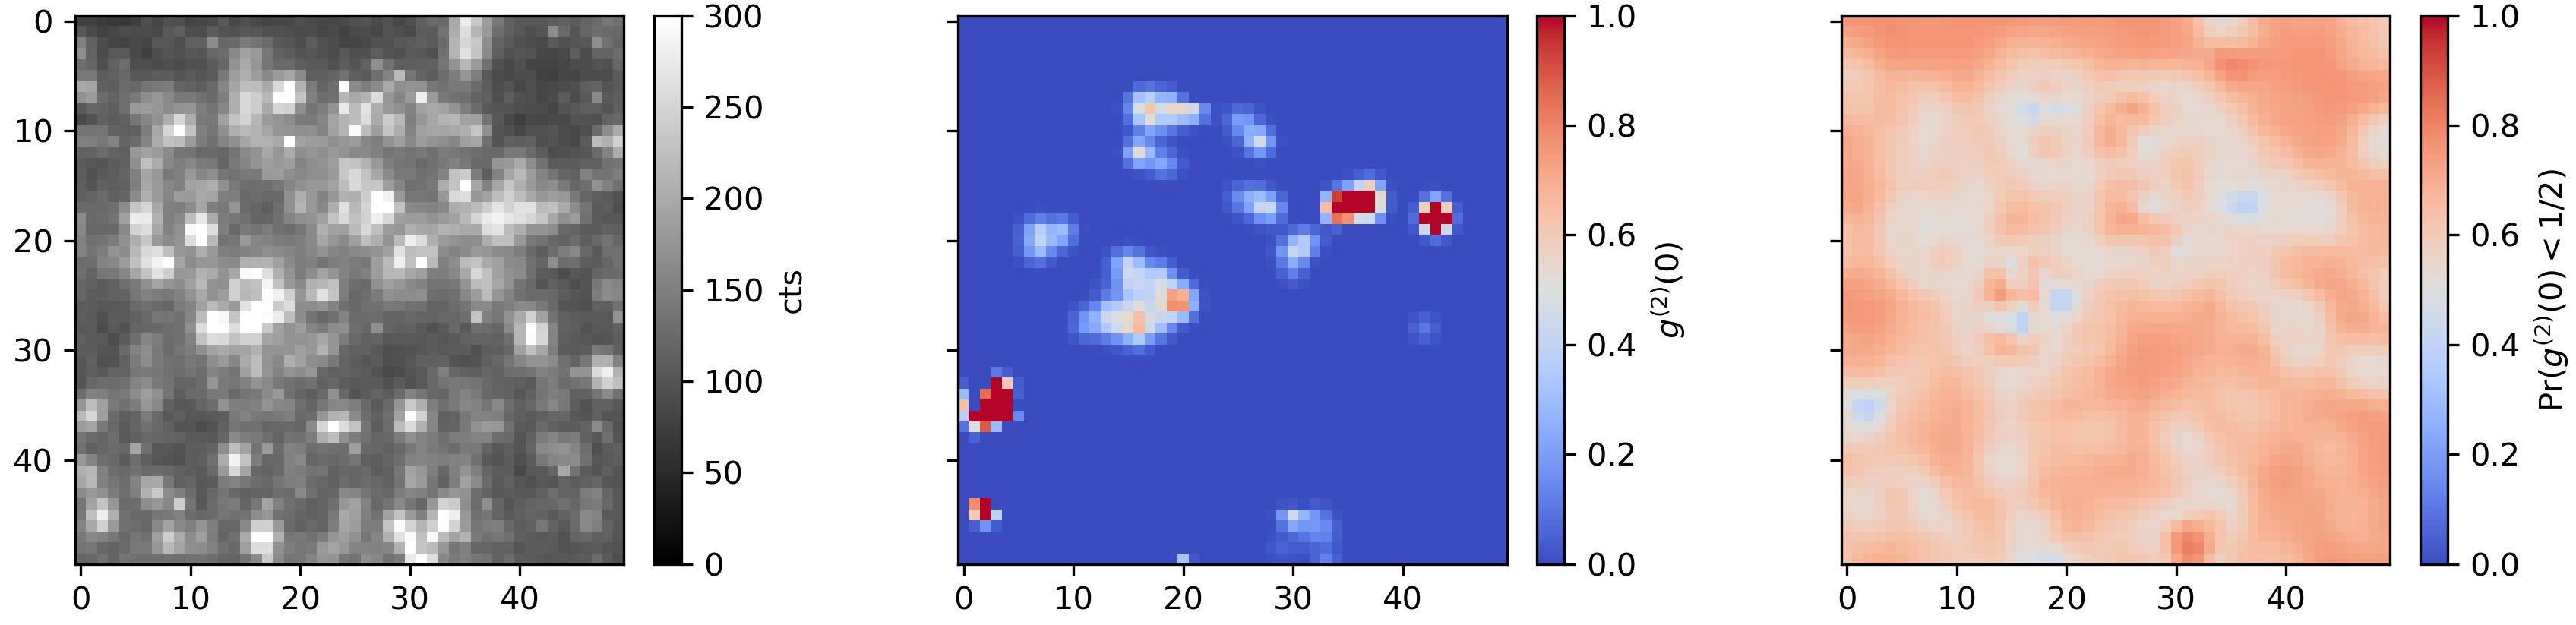
\includegraphics[width=\textwidth]{/Users/cwseitz/git/cwseitz.github.io/docs/phd/brd4/brd4/media/Figure-2.png}
\caption{\textbf{Expression of constitutively phosphorylated BRD4 compacts nucleosome nanodomains}. (a,b) Direct stochastic optical reconstruction microscopy (dSTORM) imaging strategy of single nucleosomes and an examples super-resolution image. (c) Two-color image of super-resolved H2B-JF646 with diffraction-limited GFP-tagged BRD4. (d) Besag’s L-function for various BRD4 mutants. All scalebars 3um.}
\end{figure}

\subsection{Heteropolymer model}

To interpret our experimental findings, we adopt a heteropolymer chromatin model to capture the interaction of chromatin with multivalent BRD4-like binders (Figure 4a). The heteropolymer consists of a coarse-grained bead-and-spring chain composed of $N_b=200$ beads, connected by harmonic bonds with equilibrium length $r_0$ whose energy is defined as

\begin{equation*}
U_{AB}(r_{ij})=\frac{\kappa}{2}(\lvert r_{ij}\lvert-r_0)^2
\end{equation*}

where $r_{ij}$ is a vector connecting the center of a bead of type $i$ to a bead of type $j$ and $i,j \in (A,B)$. In all simulations, we assume $\kappa=90k_{B}T{r_0}^2$ where $k_{B}$ is Boltzmann’s constant and $r_0=200$nm. Random beads in the chain are selected to represent locally unacetylated (A-type particles) and acetylated chromatin (B-type particles).  B-type particles undergo multivalent interactions with a third group of C-type particles, which can promote cross-linking of the polymer. We presume a Bernoulli probably of $p=0.3$ for any given bead to be in an acetylated-like state. Interaction of multivalent chromatin binders with chromatin beads are then mediated by the following potential:

\begin{equation*}
U_{BC}\left(r_{ij}\right)=\epsilon\left(1-\left(\frac{\lvert r_{ij}\lvert}{R_0}\right)^2\right)^3
\end{equation*}

where $R_0=200$nm. The potential $U_{BC}$ is considered over a domain $0\leq\lvert r_{ij}\lvert\leq 2 R_0$ In all simulations, ten replicates were run for each condition tested. A and B type particles within the chromatin polymer have repulsive interactions with $\epsilon = +10k_{B}T$. Binding energy of the acetylated beads with binders was varied with $\epsilon_{I} = 0 k_{B}T,\epsilon_{II} = -20k_{B}T,\epsilon{III}=-40k_{B}T$ (Figure 4b). The dynamics of chromatin chains are approximated by Brownian dynamics within a cubic box with side length of 10um and periodic boundary conditions. Brownian dynamics follows the stochastic differential equation.

\begin{figure}[t]
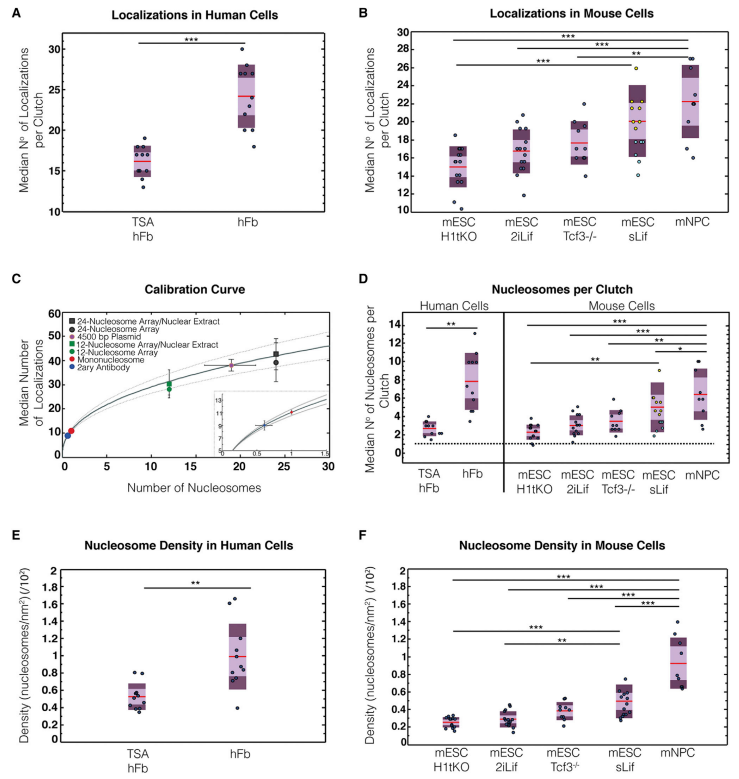
\includegraphics[width=\textwidth]{/Users/cwseitz/git/cwseitz.github.io/docs/phd/brd4/brd4/media/Figure-3.png}
\caption{\textbf{BRD4 mutants reduce single nucleosome dynamics in living cells}. (a,b) Sparse labeling of single nucleosomes in a living Hela cell (scalebar 5um). (c) Average mean squared displacement (MSD) of single nucleosomes for wild-type and mutated BRD4, error bars represent the standard error of the mean. (d) Kernel density estimates of the MSD distribution at representative lag times. }
\end{figure}

\begin{table}[h!]
\centering
\begin{tabular}{|c|c|}
\hline
\textbf{Parameter} & \textbf{Value} \\ \hline
Bond Length ($\sigma$) & $200 \times 10^{-9}$ m \\ \hline
Cutoff Distance & $500 \times 10^{-9}$ m \\ \hline
Spring Constant ($\kappa$) & 90.0 $k_{B}T/\sigma^2$ \\ \hline
Neighbor Distance & $500 \times 10^{-9}$ m \\ \hline
Damping Coefficient ($\gamma$) & $10^{-7}$ \\ \hline
Time Step & $10^{-4}$s\\ \hline
Number of Time Steps & $10^4$ \\ \hline
Number of Atoms & 200 \\ \hline
\end{tabular}
\caption{\textbf{Multivalent binder model parameters}}
\end{table}

\begin{equation*}
\dot{\bold{r}} = \gamma^{-1}\nabla U(\bold{r}) +\sqrt{2 k_{B}T}\gamma^{-1/2}\xi(t)
\end{equation*}

where $\gamma$ is a diagonal friction tensor and $\xi(t)$ is a three-dimensional delta-correlated white noise $\langle \xi(t)\xi(t+\tau)  = \delta(t,t+\tau)$. Integrating the Brownian dynamics showed an overall reduction of the variance of the diffusion coefficient $D$ of single beads, and linear scaling of the diffusion coefficient with respect to temperature (Figure 4e).

\section{Discussion}

Our data support the model that phosphorylated and unphosphorylated BRD4 form different molecular associations in the nucleus. BRD4 nuclear localization is only weakly affected by bromodomain inhibition with monovalent BET inhibitors, while exposure to phase separation inhibitors such as 1,6 Hexanediol have a significant effect on BRD4 localization in the nucleus11. Therefore, nascent BRD4 condensates are likely seeded by unphosphorylated BRD4, followed by CK2-mediated phosphorylation, promoting chromatin interactions mediated by phosphorylated form. The stable dimeric interaction and binding of phosphorylated BRD4 to acetylated chromatin would then mediate control of the chromatin architecture by promoting cross-linking of the chromatin fiber and acting a molecular ‘bridge’ between transcriptional condensates with chromatin. Concurrently, reduced diffusivity of single nucleosomes with no overall change in NN compaction (cross-linking) in the unphosphorylated mutant is a natural result of molecular crowding resulting from overexpression of a constitutively phase separating protein, capable of multivalent interactions. 

\section{Materials and Methods}

\subsection{Cell lines, cell culture conditions, and transfection}

Hela cells were cultured in DMEM supplemented with 10 percent fetal bovine serum (Gibco) at 37C 5 percent CO2 in a humidified incubator. Cultures were tested routinely for mycoplasma contamination; all tests were negative. For super-resolution experiments, cells were seeded in a 35mm FluoroDish (WPI), and transiently transfected using Lipofectamine 3000 with pBREBACK-H2BHalo plasmid (Addgene plasmid 91564) (ThermoFisher), pcDNA5-Flag-BRD4-7A (Addgene Plasmid 90006), pcDNA5-Flag-BRD4-7D (Addgene Plasmid 90007), pCDNA5-Flag-BRD4-BD (Addgene Plasmid 90005), pcDNA5-Flag-BRD4-WT (Addgene Plasmid 90331)

\subsection{Super-resolution imaging of nucleosome nanodomains in living cells}

After transient transfection, H2B-Halotag Hela cells were incubated with 3pM JF646 HaloTag ligand overnight. Cells were imaged in a dSTORM photoswitching buffer containing 100mM MEA, 50 ug/ml Glucose Oxidase, and 3.4 mg/ml Catalase (Sigma). Buffer pH was adjusted to ~8 using HCl. Movies were collected using a custom Olympus IX83 microscope body equipped with an Olympus 60X 1.25NA oil-immersion objective. During imaging cells were maintained at 37C and 5 percent CO2 in a stage top incubator (Tokai Hit). Images were projected onto an ORCA-Fusion sCMOS camera (Hamamatsu) and 2000 frames were captured at 100fps. The microscope was controlled using Micromanager software. HaloTag-JF646 molecules were imaged using oblique illumination with a 640nm laser (Excelitas) held at 20mW, as measured at the back focal plane of the objective. Super resolution reconstructions were obtained using the ThunderSTORM ImageJ plugin. Background signal was subtracted using a rolling ball filter with radius of 10 pixels. Spots were fit using an integrated Gaussian point spread function model with maximum likelihood estimation \parencite{Smith2010,Huang2013}. Experimental conditions for single molecule tracking are nearly identical. However, H2B-Halotag Hela cells were incubated with 3pM JF646 HaloTag ligand. HaloTag-JF646 molecules were illuminated at 10mW, 100 frames were captured at 10fps. 

\begin{equation*}
K(r) =\frac{a}{n(n-1)}\sum_{ij}{I(d_{ij}\ \le r)}\;\;\; L(r)\ \sqrt{\frac{K(r)}{\pi}}
\end{equation*}

Precise x,y positions of the fluorophores are obtained, Besag’s L-function L(r) is used to analyze the clustering. The L-function is the following transformation of Ripley’s K-function K(r) 


where $a$ is the area of the window, $r$ is the distance between, $n$ is the number of data points and the sum is taken over all pairs of fit coordinates as shown in equation XXX. The indicator function is given by $I(d_{ij}\le r)$ and equals 1 if the distance is less than or equal to $r$. To measure degree of clustering, we use $L(r)-r$, which measures the deviation of a point pattern from complete spatial randomness (CSR). 

\subsection{Colocalization of BRD4 mutants with nucleosome nanodomains}

We colocalize FLAG-tagged 7A/7D BRD4 mutants with nucleosome nanodomains by simultaneous FLAG immunofluorescence with imaging of sparsely labeled of H2B-JF646. Puncta were detected in both channels using the Laplacian of Gaussian (LoG) detection algorithm to generate a multi-type point pattern. We then computed the nearest neighbor distance distribution function $G(r)$, which is the cumulative distribution function of the distance from a random H2B-JF646 puncta to the nearest BRD4-FLAG puncta. This function was computed for each cell, and then averaged over $N=20$ cells for each mutant to obtain $G(r)$. The averaged value is reported alongside the theoretical $G(r)$ under complete spatial randomness

\begin{equation*}
G(r)=\ 1-e^{-\lambda\pi r^2}
\end{equation*}

Where $\lambda$ is the expected number of points per unit area. 

\subsection{Single molecule tracking}

Nucleosomes were localized using an integrated Gaussian point spread function model with maximum likelihood estimation \parencite{Smith2010,Huang2013} and tracked using TrackPy Python software.  Trajectories lasting less than 80 frames were removed from further analysis. The individual mean squared displacement (MSD) is computed as $\langle \Delta r^{2}\rangle = \frac{1}{\lvert S_{\tau}\lvert}\sum_{\Delta r \in S_{\tau}}(\Delta r)^{2}$
where $S_\tau$ is the set of all displacements in a time interval $\tau$. The diffusion coefficient for both simulations as well as experimental data was computed by linear regression of the formula $\log\langle \Delta r^{2}\rangle  = \log 4D + \alpha \log \tau$

\subsection{Immunofluorescence}
Cells grown in 35mm dishes were fixed with Formaldehyde in 1xPBS at 37C incubator for 20 minutes, and then permeabilized with 0.3 percent (v/v) Triton-X100 (Sigma-Aldrich) in PBS and blocked for 1h in 5 percent (w/v) nonfat dry milk at 4C. Cells were incubated overnight at 4C using primary antibodies anti-FLAG (Cell Signaling, clone XXX; 1:1000), and anti-BRD4 (Cell Signaling, clone E2A7X; 1:1000)  in blocker. Secondary antibodies for BRD4 (Cell Signaling Anti-Mouse IgG-Alexa488, 1:1000) were used. 

\subsection{Immunoblotting}
Cells were washed and lysis buffer added (RIPA buffer: PMSF: protease inhibitor cocktail: orthovanadate=100:1:2:1). Cells were then scraped and sonicated for 15 seconds using an ultrasonic homogenizer. Lysate was centrifuged at high speed (13200r/min) for 15 minutes at 4C to pellet the cellular debris. Total protein concentration was determined by a BCA Protein Assay Kit (Pierce). For electrophoresis, protein samples were prepared according to a protein-4x loading buffer (containing DTT) ratio of 3:1, 4x loading buffer containing DTT was diluted with 3 aliquots of protein sample. The sample was mixed and heated at 95C for 5 min, followed by vortex and centrifuge. After running the gel, it was removed from the cassette and assembled inside the Trans-Blot Turbo Transfer System cassette. Transfer was run at 2.5A and 25V for 7mins. The sample was then blocked for at least 1 hour using 5 percent skim milk blocking solution prepared with PBS in RT. Primary FLAG antibody was diluted in PBST with 3 percent skim milk (1:500) and incubated at 4C overnight. The secondary antibody (Licor Anti-Mouse IgG- IRDye 800CW) was diluted in PBST with 3 percent skim milk (1:5000) and placed on a rocker and incubated at RT for 45min. Western blots on Nitrocellulose membranes were scanned using the Odyssey fluorescence scanning system software.

